
% Does not currently include transfer plots and ODIF
% Will change considerably once added (focus on transfer capabilities, integrate into sdtf draft)

\section{Gaussian XOR Two Class Classification} In each Gaussian XOR two class classification  experiment, we compare generalization errors of \SDT~and \SDF~to HT and MF. Class 0 is drawn from two Gaussians with means $\pm [0.5,0.5]^\mathsf{T}$, and variances proportional to the identity matrix. Class 1 is drawn from two Gaussians with  means $\pm [0.5,-0.5]^\mathsf{T}$, and variances proportional to the identity matrix. We sample 750 times from XOR, followed by 750 samples of a variation of XOR (Gaussian Rotated XOR (R-XOR) or Gaussian Exclusive NOR (XNOR)), followed by an additional 750 samples of XOR. Data are introduced in batches of 25 samples at a time. These 2,250 samples comprise the training data and an additional 1,000 hold out samples comprise the testing data. Generalization errors are averaged over 50 repetitions.

\subsection{Gaussian R-XOR} Gaussian R-XOR has the same distribution as Gaussian XOR, but with the class labels rotated by $45^\circ$. \SDF~and MF outperform \SDT~and HT when trained only on XOR data and tested on XOR data. As R-XOR data are introduced, MF outperforms all other classifiers on XOR data until additional XOR data are introduced and \SDF~and \SDT~then outperform MF. When tested on R-XOR data, all classifiers perform at chance when exposed to only XOR data. As R-XOR data are introduced, \SDT~and \SDF~ outperform both HT and MF on R-XOR data. \SDF~and \SDT~again both approach chance when additional XOR data are introduced and HT and MF generalization error also increases.

\begin{figure}[!htb]
  \centering
  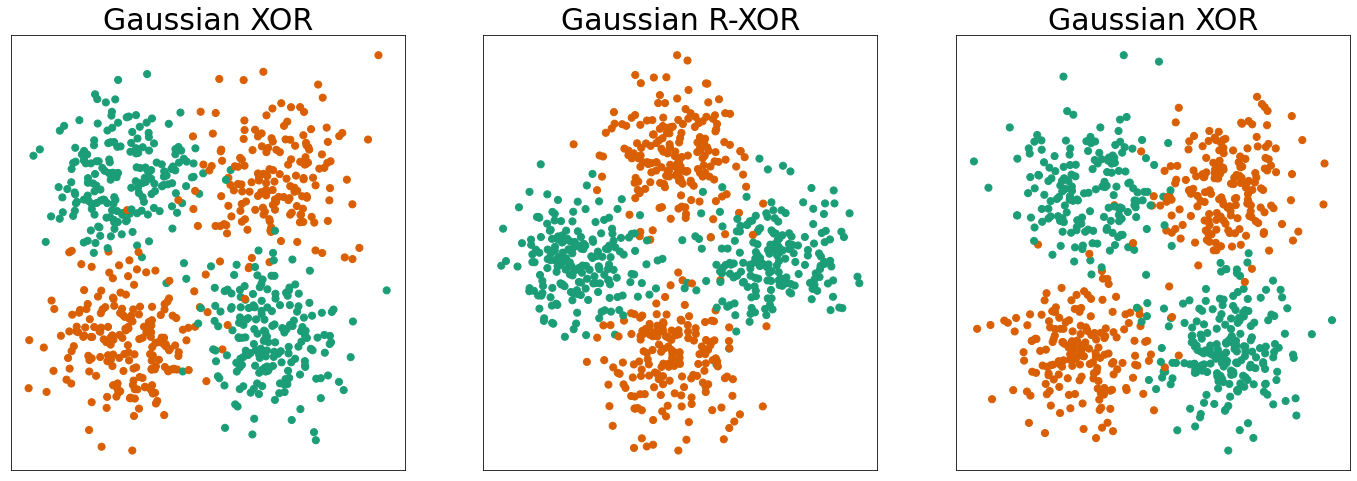
\includegraphics[width=1.0\textwidth]{XOR_RXOR_data.png}
  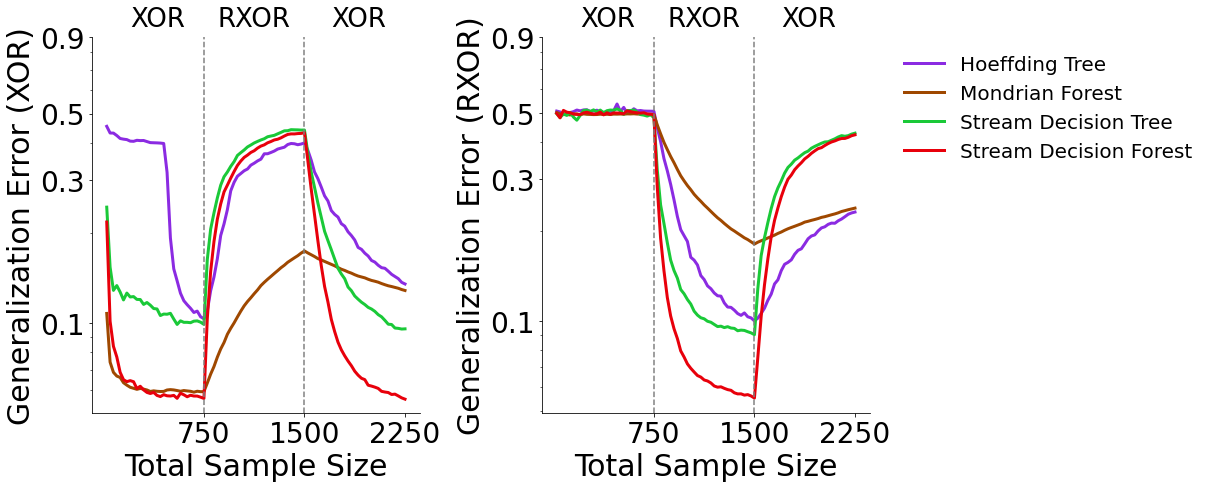
\includegraphics[width=1.0\textwidth]{XOR_RXOR_results.png}
    \caption{750 samples from Gaussian XOR \textbf{(top left)}, 750 samples from Gaussian R-XOR \textbf{(top center)}, and 750 additional samples of Gaussian XOR \textbf{(top right)}. Generalization errors on XOR \textbf{(bottom left)} and R-XOR \textbf{(bottom right)} data averaged over 50 repetitions. 
    }
  \label{fig:rxor}
\end{figure}

\subsection{Gaussian XNOR}Gaussian XNOR has the same distribution as Gaussian XOR, but with the class labels rotated $90^\circ$. 

\begin{figure}[!htb]
  \centering
  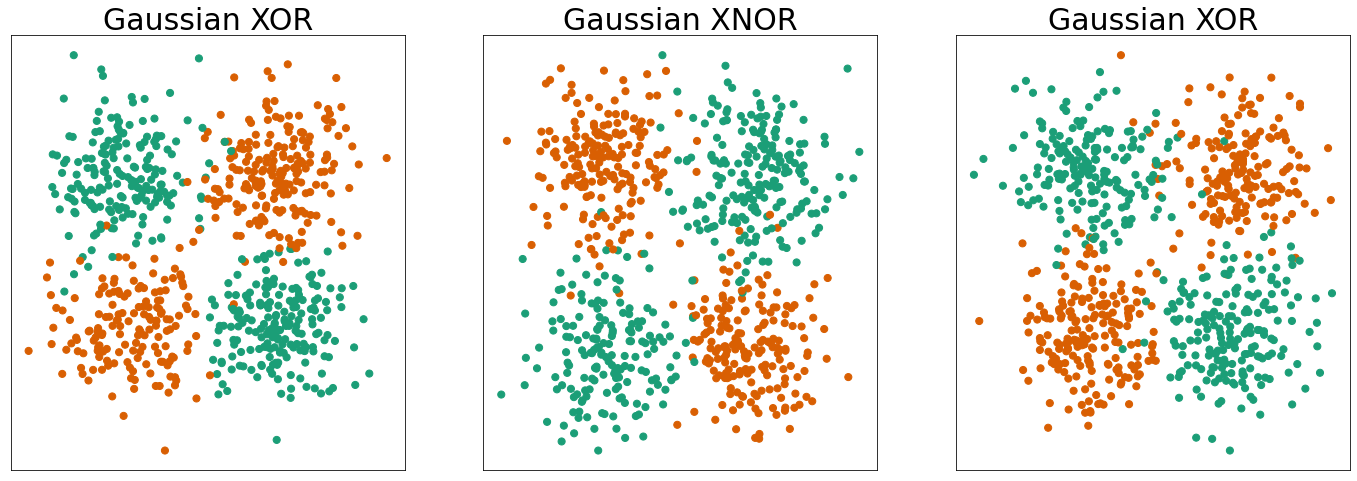
\includegraphics[width=1.0\textwidth]{XOR_XNOR_data.png}
  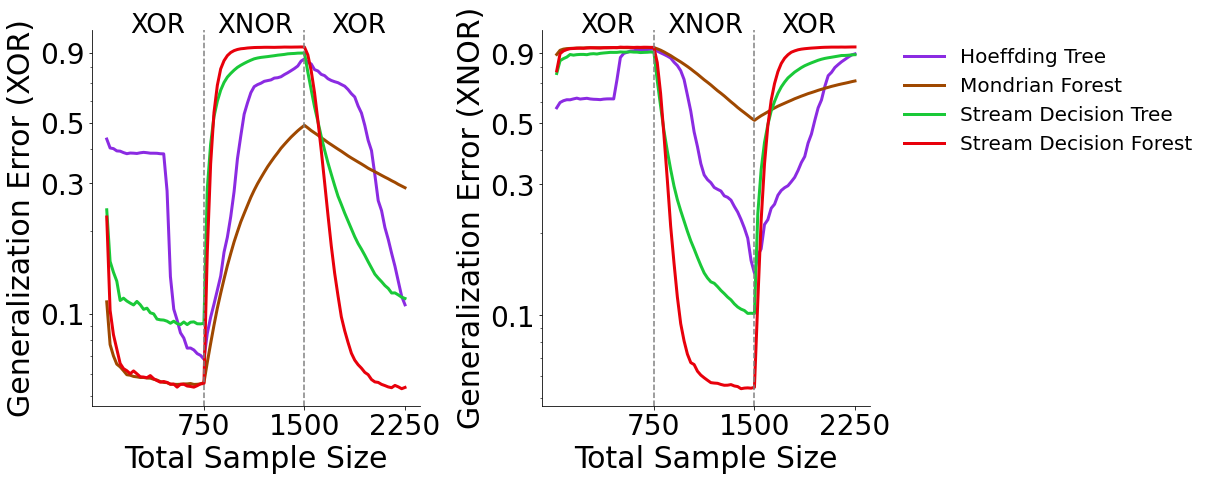
\includegraphics[width=1.0\textwidth]{XOR_XNOR_results.png}
    \caption{750 samples from Gaussian XOR \textbf{(top left)}, 750 samples from Gaussian XNOR \textbf{(top center)}, and 750 additional samples of Gaussian XOR \textbf{(top right)}. Generalization errors on XOR \textbf{(bottom left)} and XNOR \textbf{(bottom right)} data averaged over 50 repetitions. 
  }
  \label{fig:xnor}
\end{figure}
